\documentclass[11pt]{article}
\usepackage{geometry}                % See geometry.pdf to learn the layout
\usepackage{graphicx}
\usepackage{amssymb}
\usepackage{epstopdf}

\title{Compte-rendu du TEA n°3}
\author{\textsc{Valentin GAUTHIER}\\ Alexandre TORRES--LEGUET}

\begin{document}
\maketitle

\section{Introduction}
%présentation du problème, le contexte

\quad \quad Ce compte-rendu présente le travail réalisé dans le cadre du TEA 3 de l'enseignement d'AAP, qui se concentre sur le tri rapide et le tri fusion en \textsc{C}.
 
Nous avons vu en TD le principe de fonctionnement et le code de ces tris en \textsc{C}, notre tâche a alors été dans un premier temps d'adapter ce travail afin de le rendre compatible avec les outils de création de graphiques, i.e. avec la structure de données \texttt{T\textunderscore data}. 

Dans un second temps, nous avons implémenté les fonctions \texttt{fusionsort} et \texttt{quicksort} qui respectent le même prototype que la fonction \texttt{qsort} disponible nativement dans \textsc{C}. (sous réserve d'inclure \texttt{stdlib.h})

Enfin, nous avons implémenter le tri fusion sur des listes chaînées.

\section{Développement}
%organisation du programme
%organisation du groupe (qui a fait quoi)
%difficultés

\subsection{Tri fusion}

\quad \quad Le dossier \texttt{tri\textunderscore fusion} recense notre travail relatif au tri fusion sur un tableau. \\

Pour cette partie, la première partie du travail a été de transformer la fonction d'en-tête

$$
\texttt{void triFusion(T\textunderscore elt t [], int debut, int fin)}
$$

en la fonction

$$
\texttt{void triFusion(T\textunderscore data d, int n)}
$$

où \texttt{n} désigne le nombre d'éléments à considérer à partir du début du tableau passé. Il faut donc, au moment d'appeler cette deuxième fonction, envoyer la bonne partie du tableau (et non pas le tableau entier comme c'est le cas pour la première fonction). \\

Nous avons effectué ensemble la fonction \texttt{fusionsort} une fois la fonction \texttt{quicksort} implémentée car cette dernière nous a paru plus abordable pour gérer le type \texttt{void *} que l'on récupère en entrée.
Le développement de \texttt{fusionsort} a requis celui de la fonction \texttt{merge} qui permet de fusionner deux tableaux triés. Pour faire cela, nous avons été obligé de copier dans des tableaux temporaires (\texttt{L} et \texttt{R}) les données à fusionner. Nous aidant des considérations faites pendant le développement de \texttt{quicksort}, nous nous sommes beaucoup basés sur la fonction \texttt{memcpy}.

\subsection{Tri rapide}

\quad \quad Le dossier \texttt{tri\textunderscore rapide} recense notre travail relatif au tri fusion sur un tableau. \\

Le même travail de conversion a été effectué afin de rendre compatible la fonction vue en TD au type \texttt{T\textunderscore data}. \\

La fonction \texttt{quicksort} reprend les mêmes idées que \texttt{triRapide}. Cependant, l'implémentation concrète du tri a été amené à changer. La plus grosse difficulté rencontré a été que le tableau passé en entrée est de type \texttt{void *} (i.e. type non déterminé).
Cela a notamment posé un problème dans la fonction annexe \texttt{echanger} qui a pour but d'échanger 2 éléments d'un tableau. En effet, le compilateur nous empêche d'assigner une valeur à type \texttt{void *} : la solution pour pallier à cela a été d'utiliser la fonction native \texttt{memcpy} afin de ne pas avoir à assigner une valeur. 

\subsection{Tri rapide sur une liste chaînée}

\quad \quad Le dossier \texttt{tri\textunderscore fusion\textunderscore listes} recense notre travail relatif au tri fusion sur une liste chaînée.

Nous nous sommes d'abord concentré sur la fonction \texttt{couper}, qui a pour but de diviser en 2 moitié une liste chaînée. Cette fonction, au lieu de retourner 2 valeurs qui sont les têtes des 2 listes, modifie 2 pointeurs (\texttt{T\textunderscore node **head\textunderscore 1} et \texttt{T\textunderscore node **head\textunderscore 2}) qui, une fois la fonction terminée, pointeront sur les 2 listes divisées.

Voici un schéma explicatif qui montre le déroulement de cette division : 

\begin{center}
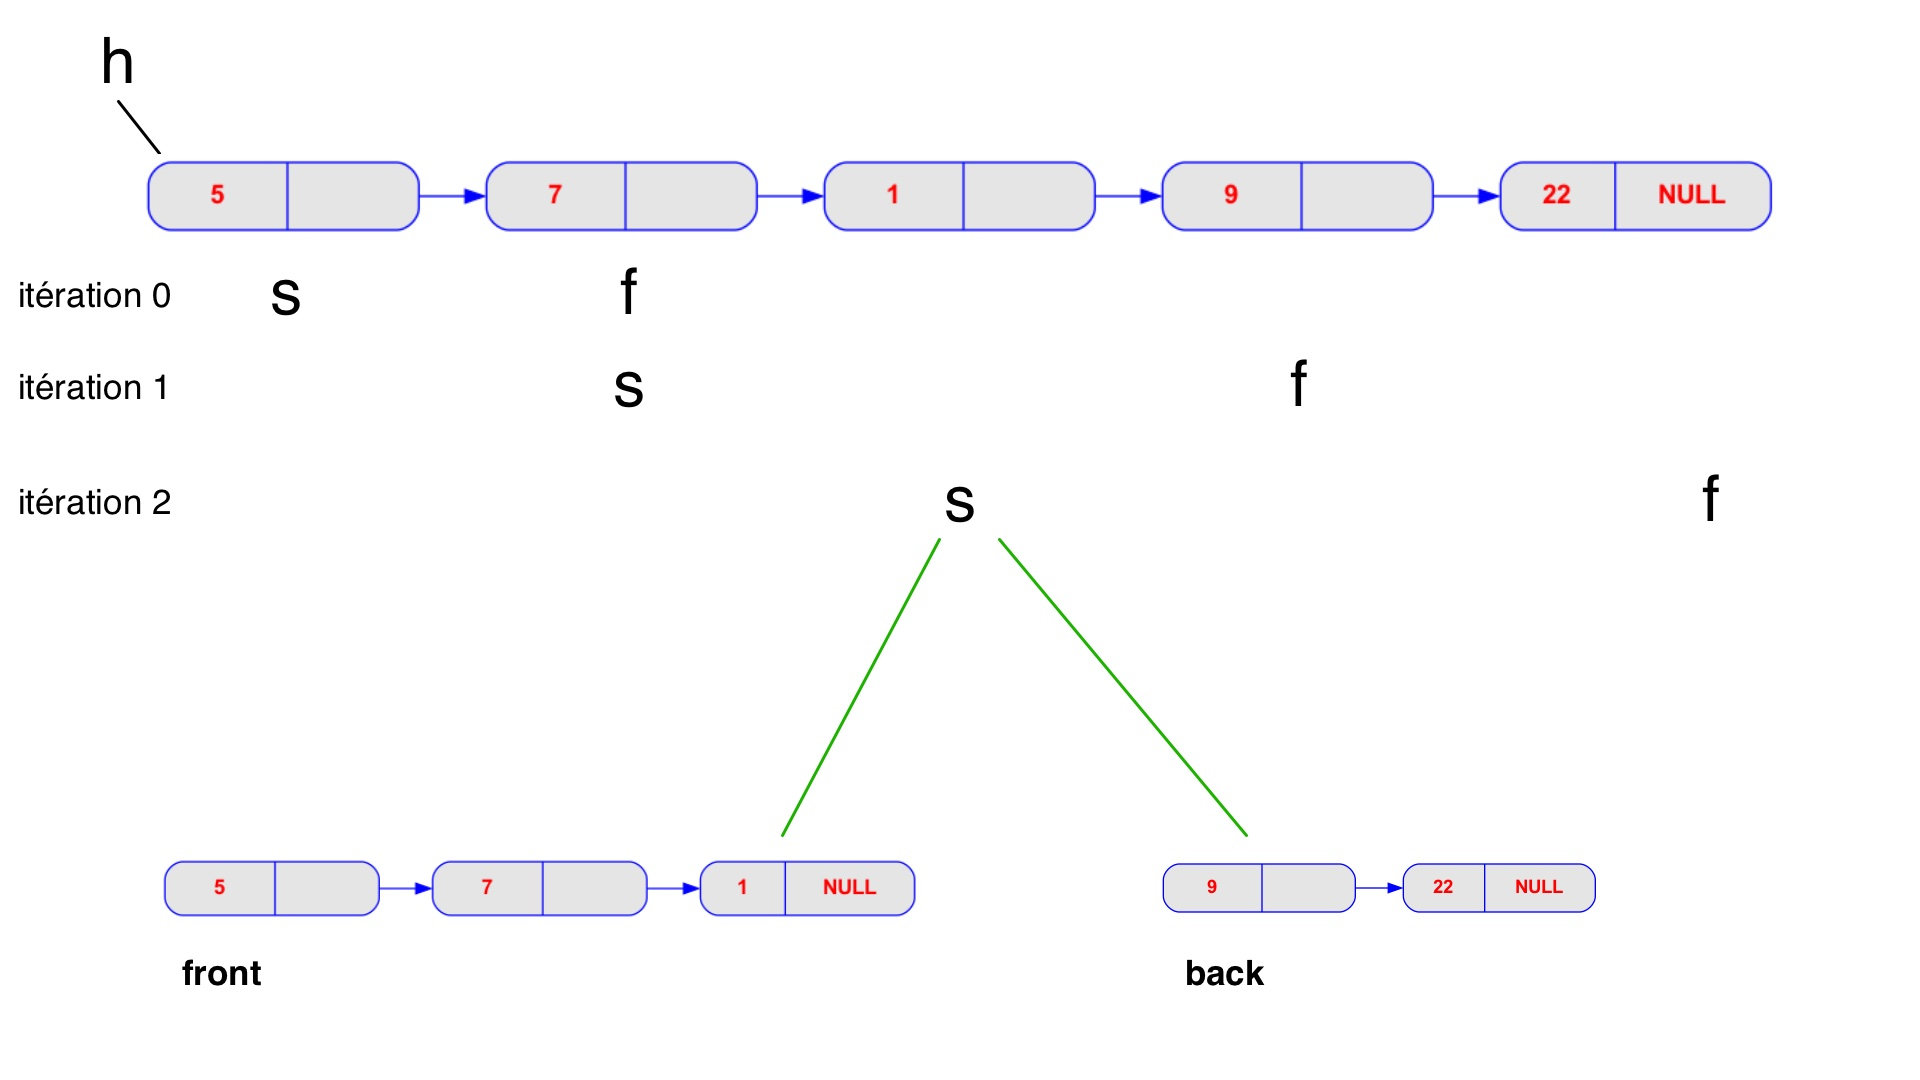
\includegraphics[scale=0.25]{images/2.jpg}
\end{center}

\texttt{s} et \texttt{f} correspondent aux variables \texttt{slow} et \texttt{fast} de notre code : ces pointeurs parcourent la liste, mais un le fait de manière "lente" (une maille à la fois) et l'autre le fait plus rapidement (deux mailles à la fois). Il s'en suit que, lorsqu'on les fait parcourir la liste, à la fin, lorsque \texttt{f} atteint le bout de la liste, \texttt{s} se trouve au milieu de la liste. On s'en sert alors pour découper la liste en deux. On peut comparer cette situation à la suivante : deux personnes montent le même escalier, et, quand la première personne monte une marche, la seconde en monte deux. Alors, lorsque la seconde personne sera arrivée en haut de l'escalier, la première en sera à la moitié. \\


La fonction \texttt{fusion} fusionne 2 listes chaînées supposées triées. Le principe est le même qu'avec le tableau : on compare les premiers éléments de chacun des deux listes à fusionner, on sélectionne le petit, puis on recommence... jusqu'à épuisement des deux listes. \\

La fonction \texttt{triFusionListes} se tâche simplement de diviser la liste d'entrée, trier récursivement les deux listes obtenues, et de les fusionner. \\

Voici un schéma permettant d'illustrer le tri fusion sur une liste chaînée :

\begin{center}
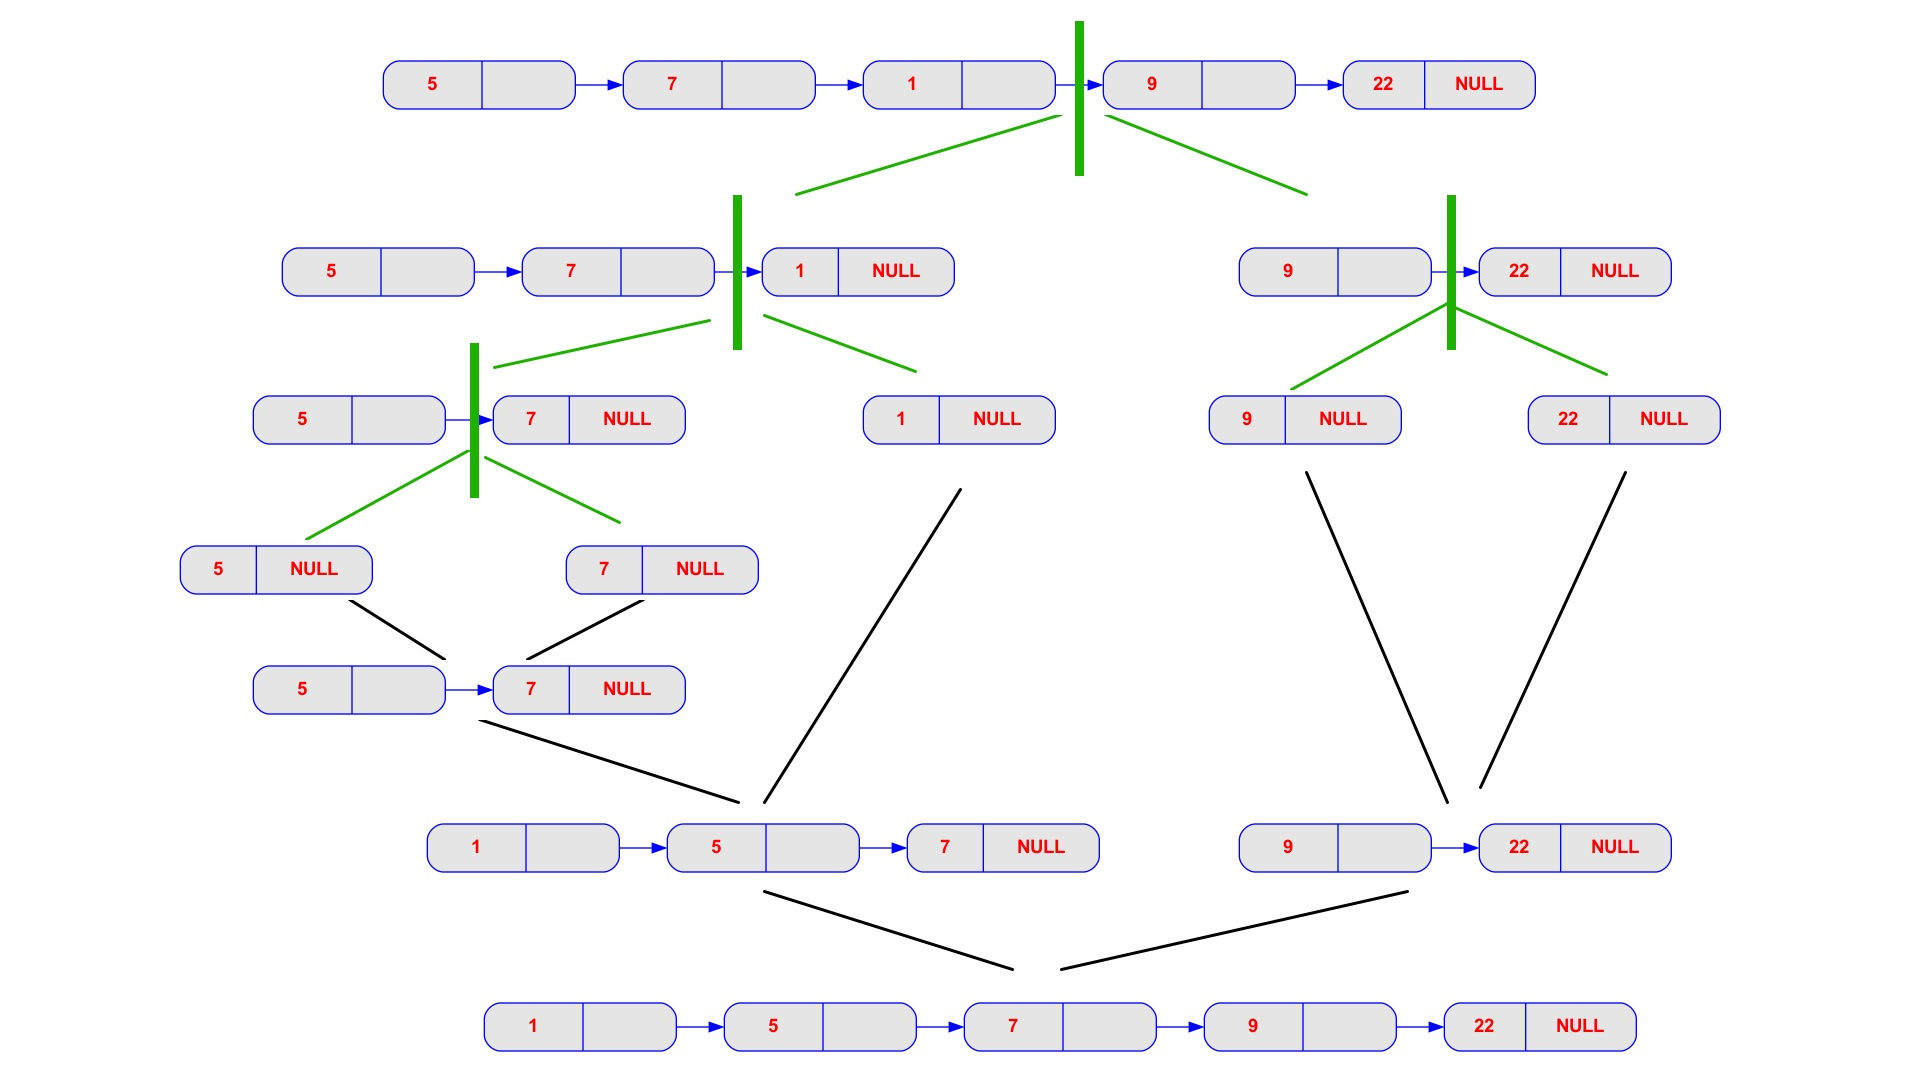
\includegraphics[scale=0.25]{images/1.jpg}
\end{center}

\subsection{Organisation - Gestion de projet}

Concernant l'organisation des tâches au sein du groupe, Valentin s'est chargé de la partie concernant le tri fusion et Alexandre celle du tri rapide. Ce travail a été opéré le week-end qui a suivi notre séance de TP du vendredi.

Enfin, au cours du début de la semaine suivante, nous avons pu nous réunir afin de réfléchir à adapter et implémenter l'algorithme de tri fusion sur une liste chaînée. Pour cela, nous sommes revenus sur la séance de TP antécédente pendant laquelle nous avions implémenté le type de liste chaînée (fichiers \texttt{list.h} et \texttt{list.c}).


\section{Résultats}
%présentation des résultats, jeux d'essais, analyse, temps d'exec...
Voici le comportement de nos algorithmes sur des tableaux de grande taille.
On observe bien un comportement quasi-linéaire pour les tris fusion et rapide sur des tableaux de nombre aléatoires.

\begin{center}
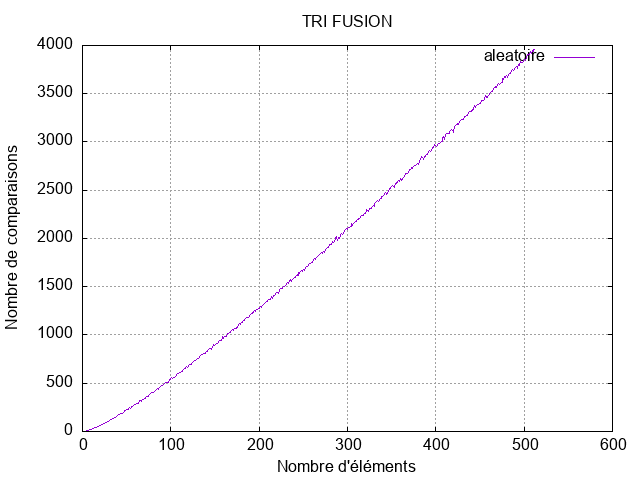
\includegraphics[scale=0.6]{images/tri_fusion_comp.png}
\end{center}

\begin{center}
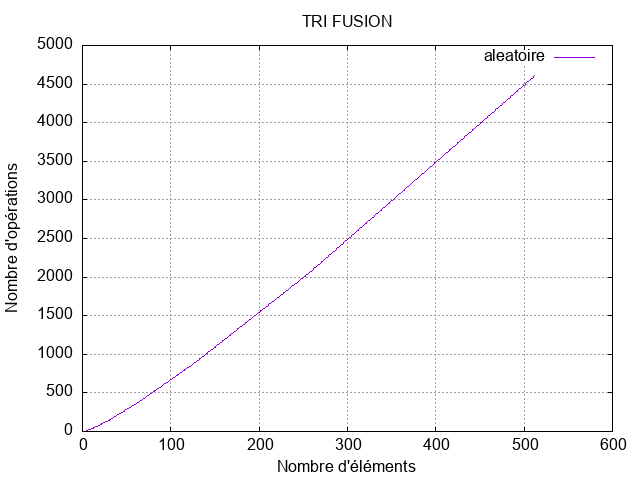
\includegraphics[scale=0.6]{images/tri_fusion_ope.png}
\end{center}

\begin{center}
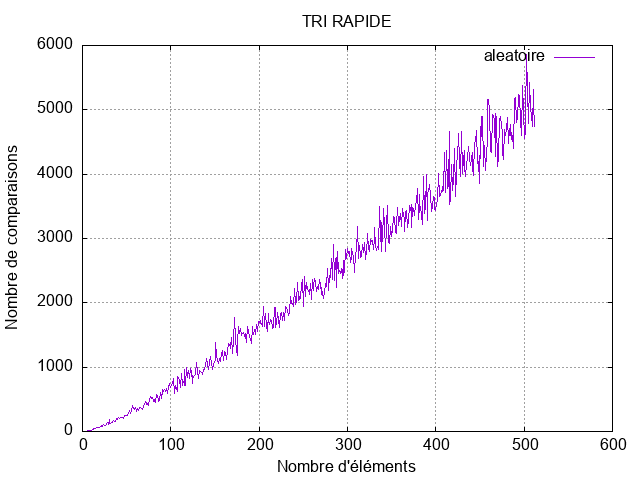
\includegraphics[scale=0.6]{images/tri_rapide_aleat.png}
\end{center}

Toutefois, le tri rapide d'un tableau ordonné laisse place à un comportement en $\Theta(n^2)$ : c'est la dégénérescence du tri rapide. En effet, le tri rapide comme nous l'avons implémenté dans un premier temps choisit pour pivot le dernier élément du tableau. Ainsi, si le tableau est déjà trié, le pivot est le nombre le plus grand du tableau : les deux sous-tableaux construits sont donc le tableau vide et le tableau contenant tous les éléments sauf le pivot : on perd donc en efficacité. 

\begin{center}
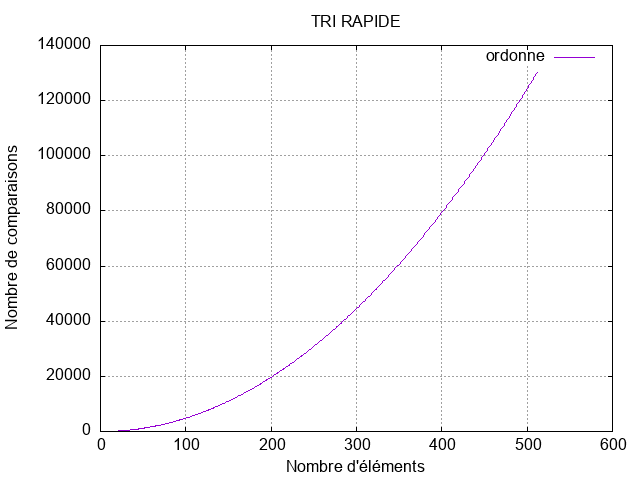
\includegraphics[scale=0.6]{images/tri_rapide_degen.png}
\end{center}

L'idée pour pallier à ce problème est de choisir le pivot tel que les deux sous-tableaux soient équilibrés. Une solution simple est de prendre le pivot comme étant l'élément du milieu. C'est ce que nous avons fait et voici le résultat :

\begin{center}
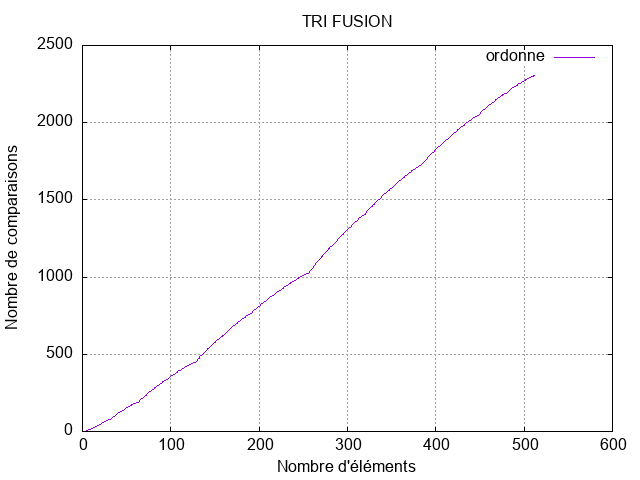
\includegraphics[scale=0.6]{images/tri_rapide_fixed.png}
\end{center}

Une autre méthode consiste à prendre 3 éléments du tableau au hasard, et à choisir l'élément médian parmi ces 3. Nous n'avons pas testé cette technique.


Nous avons enfin comparé nos implémentations des tris rapide et fusion avec la fonction \texttt{qsort} native de \textsc{C}. Pour cela, nous avons utilisé la bibliothèque \texttt{time} afin de mesurer le temps d'exécution de nos programmes. Les temps que l'on voit apparaître dans le tableau correspondent au tri de 100 tableaux de taille \texttt{MAX\textunderscore ELT = 250 000}.

\begin{center}
\begin{tabular}{||c c c||} 
 \hline
 \texttt{quicksort} & \texttt{fusionsort} & \texttt{qsort} \\ [0.5ex] 
 \hline\hline
11.2s & 12.1s & 4.1s \\ 
\hline
\end{tabular}
\end{center}

On remarque que l'implémentation native de $\texttt{qsort}$ bat largement nos deux implémentations.

\section{Conclusion}
%analyser les problèmes, perspectives

\quad \quad Nous avons pu, au cours de ce TEA, nous familiariser grandement avec le tri fusion et le tri rapide, ainsi que leurs performances globales. L'utilisation du tri fusion sur les listes chaînes nous a permis de nous rendre compte de l'avantage d'utiliser des listes afin de réduire l'empreinte mémoire de nos programmes.

\end{document}  
